% FlashOCC occupancy branch: encoder chain + BEVOCCHead2D detail.
\documentclass[tikz,border=8pt]{standalone}
% Shared styles for the DSB architecture diagrams.
\usepackage[T1]{fontenc}
\usepackage{graphicx}
\usetikzlibrary{arrows.meta, backgrounds, calc, fit, positioning, shapes.geometric}

\definecolor{camA}{HTML}{2A78D6}
\definecolor{lidA}{HTML}{1BAF7A}
\definecolor{fusA}{HTML}{EB6834}
\definecolor{detA}{HTML}{6250D6}
\definecolor{segA}{HTML}{0E8FA8}
\definecolor{occA}{HTML}{B5482A}
\definecolor{inkA}{HTML}{262626}
\definecolor{mutA}{HTML}{6B6B6B}

\tikzset{
  blk/.style={
    draw=inkA!70, line width=0.45pt, rounded corners=2.5pt,
    align=center, font=\small, inner sep=3pt,
    minimum height=0.95cm, text=inkA, fill=white,
  },
  cam/.style={blk, fill=camA!10, draw=camA!75},
  lid/.style={blk, fill=lidA!10, draw=lidA!75},
  fus/.style={blk, fill=fusA!12, draw=fusA!80},
  det/.style={blk, fill=detA!10, draw=detA!75},
  seg/.style={blk, fill=segA!10, draw=segA!75},
  occ/.style={blk, fill=occA!10, draw=occA!75},
  io/.style={blk, fill=black!4, draw=inkA!55},
  arr/.style={-{Stealth[length=2.2mm,width=1.6mm]}, line width=0.65pt, draw=inkA!75},
  darr/.style={arr, dashed},
  tag/.style={font=\scriptsize, text=mutA},
  grp/.style={draw=mutA!70, dashed, line width=0.6pt, rounded corners=6pt, inner sep=8pt},
  hdr/.style={font=\normalsize\bfseries, text=inkA, anchor=west},
  note/.style={font=\scriptsize, text=mutA, align=left},
}


\begin{document}
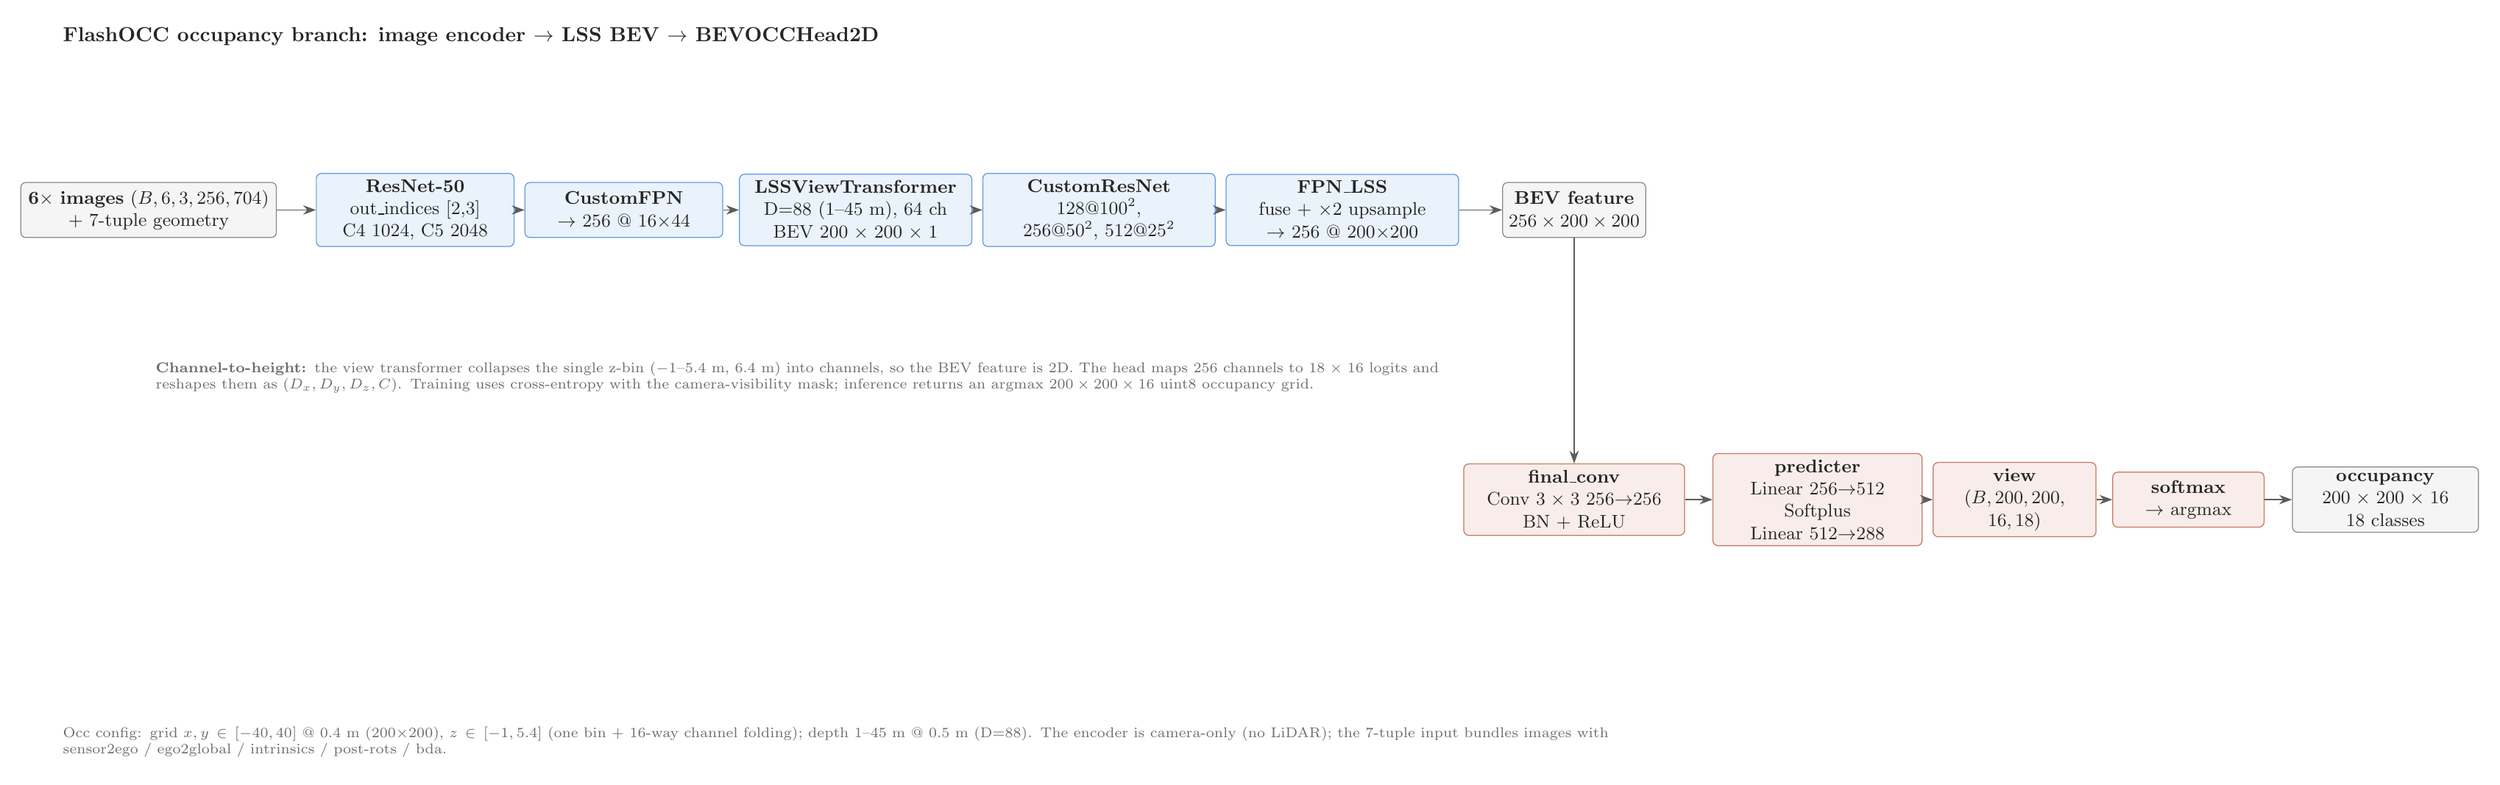
\begin{tikzpicture}

% ---------------------------------------------------------------- occ encoder
\node[io, text width=4.2cm] (in) at (0,12)
  {\textbf{6$\times$ images} $(B,6,3,256,704)$\\+ 7-tuple geometry};
\node[cam, text width=3.2cm] (r50) at (4.6,12)
  {\textbf{ResNet-50}\\out\_indices [2,3]\\C4 1024, C5 2048};
\node[cam, text width=3.2cm] (fpn) at (8.2,12)
  {\textbf{CustomFPN}\\$\to$ 256 @ 16$\times$44};
\node[cam, text width=3.8cm] (lss) at (12.2,12)
  {\textbf{LSSViewTransformer}\\D=88 (1--45 m), 64 ch\\
   BEV $200\times200\times1$};
\node[cam, text width=3.8cm] (cr) at (16.4,12)
  {\textbf{CustomResNet}\\128@100$^2$, 256@50$^2$, 512@25$^2$};
\node[cam, text width=3.8cm] (fpnlss) at (20.6,12)
  {\textbf{FPN\_LSS}\\fuse + $\times2$ upsample\\
   $\to$ 256 @ 200$\times$200};
\node[io] (bev) at (24.6,12)
  {\textbf{BEV feature}\\$256\times200\times200$};

\draw[arr] (in) -- (r50);
\draw[arr] (r50) -- (fpn);
\draw[arr] (fpn) -- (lss);
\draw[arr] (lss) -- (cr);
\draw[arr] (cr) -- (fpnlss);
\draw[arr] (fpnlss) -- (bev);

% ---------------------------------------------------------------- BEVOCCHead2D
\node[occ, text width=3.6cm] (final) at (24.6,7.0)
  {\textbf{final\_conv}\\Conv $3\times3$ 256$\to$256\\BN + ReLU};
\node[occ, text width=3.4cm] (pred) at (28.8,7.0)
  {\textbf{predicter}\\Linear 256$\to$512\\
   Softplus\\Linear 512$\to$288};
\node[occ, text width=2.6cm] (view) at (32.2,7.0)
  {\textbf{view}\\$(B,200,200,$\\$16,18)$};
\node[occ, text width=2.4cm] (arg) at (35.2,7.0)
  {\textbf{softmax}\\$\to$ argmax};
\node[io, text width=3.0cm] (out) at (38.6,7.0)
  {\textbf{occupancy}\\$200\times200\times16$\\18 classes};

\draw[arr] (bev.south) -- (final.north);
\draw[arr] (final) -- (pred);
\draw[arr] (pred) -- (view);
\draw[arr] (view) -- (arg);
\draw[arr] (arg) -- (out);

% ---------------------------------------------------------------- details / notes
\node[note, anchor=north west, text width=22.5cm] at (0,9.5)
  {\textbf{Channel-to-height:} the view transformer collapses the single z-bin
   ($-1$--$5.4$ m, 6.4 m) into channels, so the BEV feature is 2D. The head maps
   256 channels to $18\times16$ logits and reshapes them as $(D_x,D_y,D_z,C)$.
   Training uses cross-entropy with the camera-visibility mask; inference returns
   an argmax $200\times200\times16$ uint8 occupancy grid.};

\node[note, anchor=north west, text width=27cm] at (-1.6,3.2)
  {Occ config: grid $x,y\in[-40,40]$ @ 0.4 m (200$\times$200), $z\in[-1,5.4]$ (one bin + 16-way
   channel folding); depth 1--45 m @ 0.5 m (D=88). The encoder is camera-only (no LiDAR); the
   7-tuple input bundles images with sensor2ego / ego2global / intrinsics / post-rots / bda.};

\node[hdr] at (-1.6,15.0) {FlashOCC occupancy branch: image encoder $\to$ LSS BEV $\to$ BEVOCCHead2D};

\end{tikzpicture}
\end{document}
